\documentclass{article}
\usepackage{blindtext}
\usepackage[utf8]{inputenc}
\usepackage[margin=0.75in]{geometry}
\usepackage{graphicx}
\usepackage{float}
\usepackage{listings}
\graphicspath{ {./Images/} }

\providecommand{\e}[1]{\ensuremath{\times 10^{#1}}}
 
\title{CBE 710 Simulation Project}
\author{Eric O'Neill}
\date{\today}
 
\begin{document}

 
\maketitle
 
\section*{Problem 1}
 
\subsection*{Part a}
Presented here are the final configurations and graphs showing the convergence of $\frac{E}{N}$ for each of the three values of J. Along with an approximate number of Monte Carlo steps it takes to converge. The full source code can be found at the end of this doccument in Appendix A.
	\subsubsection*{$J = -2k_BT$}

	The energy per spin converges in around 20,000 Monte-Carlo steps. The figures shown below show the final configuration after 500,000 MC steps sampling the energy per particle every 500 steps and also a plot of the energy per spin versus the MC step in units of $k_BT$. For $J=-2k_BT$ the system converges to a lattice with alternating spins. The plot of energy per spin exponentially decays to a minimum energy configuration as expected. 


	\begin{figure}[H]
		\centering
		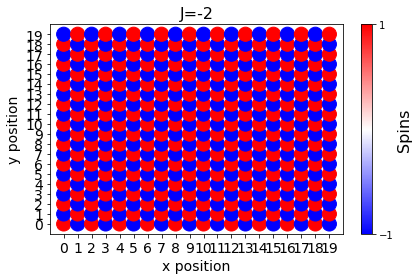
\includegraphics[scale=0.75]{J=-2}
		\caption{Final configuration after 500,000 Monte Carlo Steps}
	\end{figure}

	\begin{figure}[H]
		\centering
		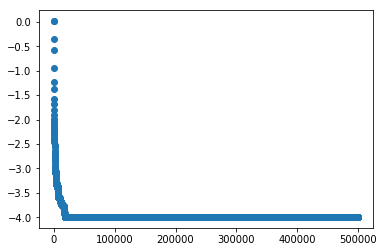
\includegraphics[scale=0.75]{J=-2b}
		\caption{Exponential decay of E/N to a constant value}
	\end{figure}

	\begin{figure}[H]
		\centering
		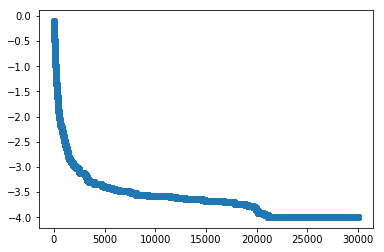
\includegraphics[scale=0.75]{J=-2c}
		\caption{Zoom in on Figure 2 to show convergence}
	\end{figure}

	\subsubsection*{$J = -0.5k_BT$}

	The energy per spin converges in around 30,000 Monte-Carlo steps. The figures shown below show the final configuration after 750,000 MC steps sampling the energy per particle every 500 steps and also a plot of the energy per spin versus the MC step in units of $k_BT$. For $J=0.5k_BT$ the system converges to a lattice with alligned spins. The lattice is does not have all spins perfectly alligned because the J value of 0.5 allows a probability to reach configurations with higher energy which have a few of the spins flipped. The energy per spin decays exponentially as well. In this case, depending on the initial state of the system and how it is sampled, the system can converge to all spins having +1 or all having -1 spins. 

	


	\begin{figure}[H]
		\centering
		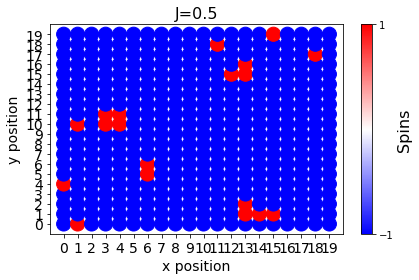
\includegraphics[scale=0.5]{J=05a.png}
		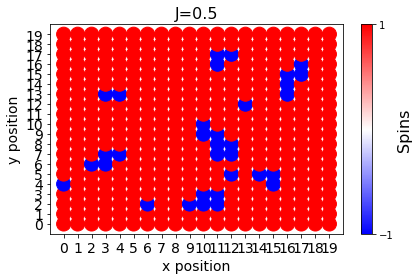
\includegraphics[scale=0.5]{J=05c.png}
		\caption{Final configurations after 750,000 Monte Carlo Steps}
	\end{figure}

	\begin{figure}[H]
		\centering
		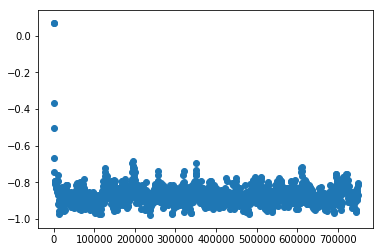
\includegraphics[scale=0.75]{J=05b}
		\caption{Exponential decay of E/N to a constant value}
	\end{figure}

	\begin{figure}[H]
		\centering
		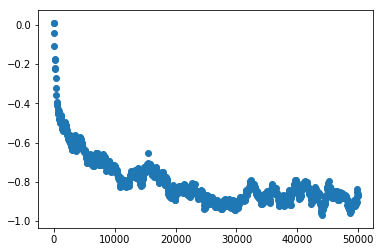
\includegraphics[scale=0.75]{J=05d}
		\caption{Zoom in on Figure 5 to show convergence}
	\end{figure}

	\subsubsection*{$J = -2k_BT$}

	The energy per spin converges in around 20,000 Monte-Carlo steps. The figures shown below show the final configuration after 500,000 MC steps sampling the energy per particle every 500 steps and also a plot of the energy per spin versus the MC step in units of $k_BT$. For $J=2k_BT$ the system converges to a lattice with alligned spins. The plot of energy per spin exponentially decays to a minimum energy configuration as expected. The $J=2$ case fully converges because the higher J value means that there is a lower probability of accepting a higher energy state. Note that in all three cases -2, 0.5, and 2, meta-stable states are possible in which spins are not perfectly alternating or there is a band of negative spins in a predominantly positive spin lattice or vice versa. Sampled over a much longer timespan, these metastable states will tend toward the most stable configurations which are shown.


	\begin{figure}[H]
		\centering
		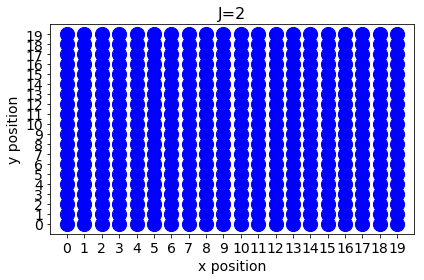
\includegraphics[scale=0.5]{J=2a}
		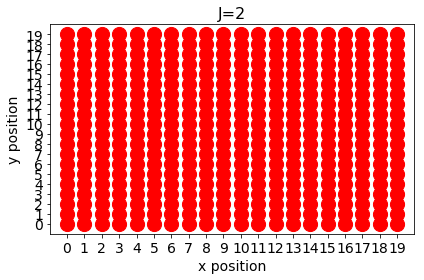
\includegraphics[scale=0.5]{J=2b}
		\caption{Final configuration after 500,000 Monte Carlo Steps}
	\end{figure}

	\begin{figure}[H]
		\centering
		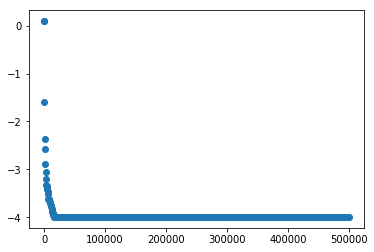
\includegraphics[scale=0.75]{J=2c}
		\caption{Exponential decay of E/N to a constant value}
	\end{figure}

	\begin{figure}[H]
		\centering
		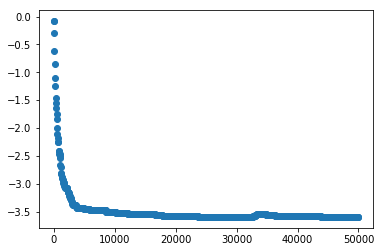
\includegraphics[scale=0.75]{J=2d}
		\caption{Zoom in on Figure 8 to show convergence}
	\end{figure}
	
 
\subsection*{Part b}
 	The magnetizations per particle plotted against the number of Monte Carlo steps for each value of J are shown below. The snapshot of the final configurations can be seen in Figure 1, Figure 4, and Figure 7. above. The equilibrium average ensamble magnetization was calculated using the following formula

 	\[\langle M \rangle = \frac{1}{Steps} \sum_{i=1}^{Steps} \sum_{i=1}^N \mu s_i\]

	\subsubsection*{$J=-2k_BT $}
		$\langle M \rangle = -2.22\e{-5} \mu$ . We expect the ensamble average magnetization to be zero because there will be an equal number of alternating positive and negative spins. The plot looks like a funnel that converges to zero. The random starting state has a non-zero magnetization, but as the simulation proceeds it comes to a steady state with zero magnetization.
		\begin{figure}[H]
			\centering
			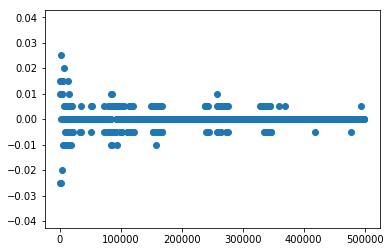
\includegraphics[scale=0.5]{J=-2m}
			\caption{Magnetization per particle for $J=-2k_BT$}
		\end{figure}

	\subsubsection*{$J=0.5k_BT $}
			$\langle M \rangle = 0.8933\mu$ or $\langle M \rangle = -0.8944\mu$ . The magnetization per particle approaches positive or negative one. Once the system reaches its equilibrium value, the low value of J leads to a higher probablity of accepting a higher energy state and produces fluctuations around the equilibrium so the ensamble average magnetization is not exactly one. 

			\begin{figure}[H]
				\centering
				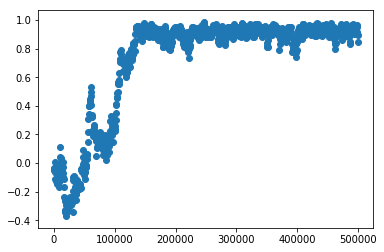
\includegraphics[scale=0.5]{J=05m1}
				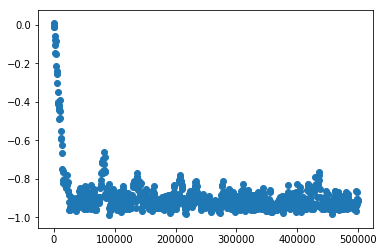
\includegraphics[scale=0.5]{J=05m2}
				\caption{Magnetization per particle for $J=0.5k_BT$}
			\end{figure}

	\subsubsection*{$J=2k_BT $}
			$\langle M \rangle = 0.9912\mu$ or $\langle M \rangle = -0.9682\mu$ . The magnetization per particle rapidly approaches positive or negative one. Once the system reaches equilibrium, the magnetization per particle stays at plus or minus one. Therefore, the ensamble average magnetization will approach one the more simulation steps are used. 

			\begin{figure}[H]
				\centering
				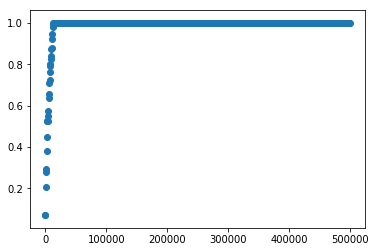
\includegraphics[scale=0.5]{J=2m1}
				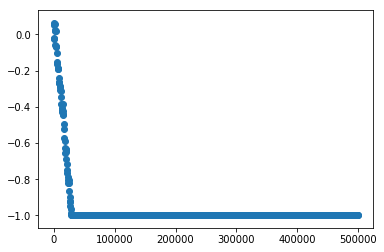
\includegraphics[scale=0.5]{J=2m2}
				\caption{Magnetization per particle for $J=-2k_BT$}
			\end{figure}






\subsection*{Part c}

	We define the average fluctuations of energy as:

	\[\langle (\delta E)^2\rangle = \langle (E- \langle E \rangle )^2 \rangle\]
	\[= \langle E^2 \rangle - \langle E \rangle ^2\]


	\noindent and because $\langle E \rangle = - (\frac{\partial \ln Z}{\partial \beta})_{N,V}$, 

	\[\langle(\delta E)^2 \rangle = k_B T^2 C_V\]

	\[C_V = \frac{\langle(\delta E)^2 \rangle}{k_B T^2}\]

	\noindent We can claculate $\langle E^2 \rangle - \langle E \rangle ^2$ in our simulation by taking the variance. However we have to be careful to only sample after the simulation is at steady state (MC steps to reach steady state are described in part a). To make sure we get an accurate value of $C_V$, we will take 1,000,000 steps and calculate fluctuations after 50,000 Monte Carlo steps for each value of J.

	\begin{center}
	\begin{tabular}{ c | c }

	J Value & $C_V$ \\
	\hline
	$-2 k_BT$ & 0 $k_B$ \\
	$0.5 k_BT$ & 260.37 $k_B$ \\
	$2 k_BT$ & 0 $k_B$ \\
	\hline

	\end{tabular}
	\end{center}


\subsection*{Part d}

	The addition of a weak magnetic field would make the spins alligning in a positive direction a more favorable configuration.

	\[ E_\nu = -\sum_i^N k_BTs_i - \frac{J}{2} \sum_i^N\sum_j^`s_is_j \]
	

	The more $s_i$ and $s_j$ in the above equation that are positive makes the overall energy more negative (if J is positive) and thus more favorable. Because more spins will be alligned in the positive direction the magnetization $M=\sum_{i=1}^N \mu s_i$ will approach positive $\mu N$. If J is negative, it will depend on which term in the energy equation dominates which will determine if the spins will allign (if the field term dominates) or if they alternate (if the interaction term dominates).

\newpage

\section*{Problem 2}

\subsection*{Part a}

	For the simulation, five trials were run on a temperature range of 0.1 to 6.0 $J/k_B$ (increment 0.1) with 1,000,000 steps sampled every 500 steps. Plots of the average values over the five trials of $|\langle M \rangle / N|$ and $C_V$ can be seen in figures 13 and 14 below.

		\begin{figure}[H]
				\centering
				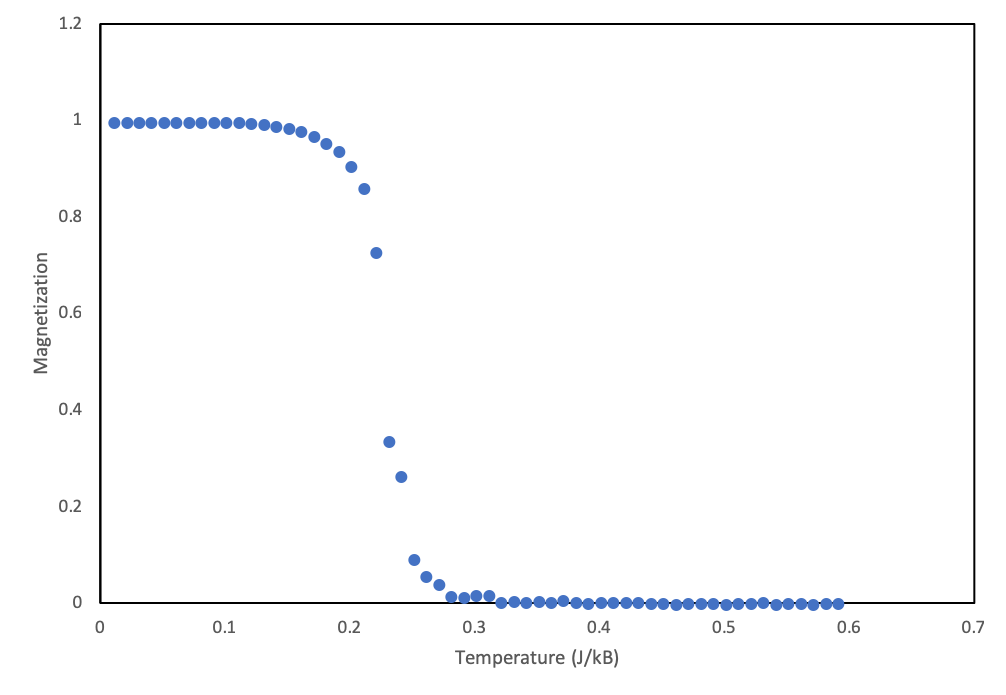
\includegraphics[scale=0.5]{Mag2}
				\caption{Absolute value of ensamble average Magnetization per particle versus temperature}
		\end{figure}

		\begin{figure}[H]
				\centering
				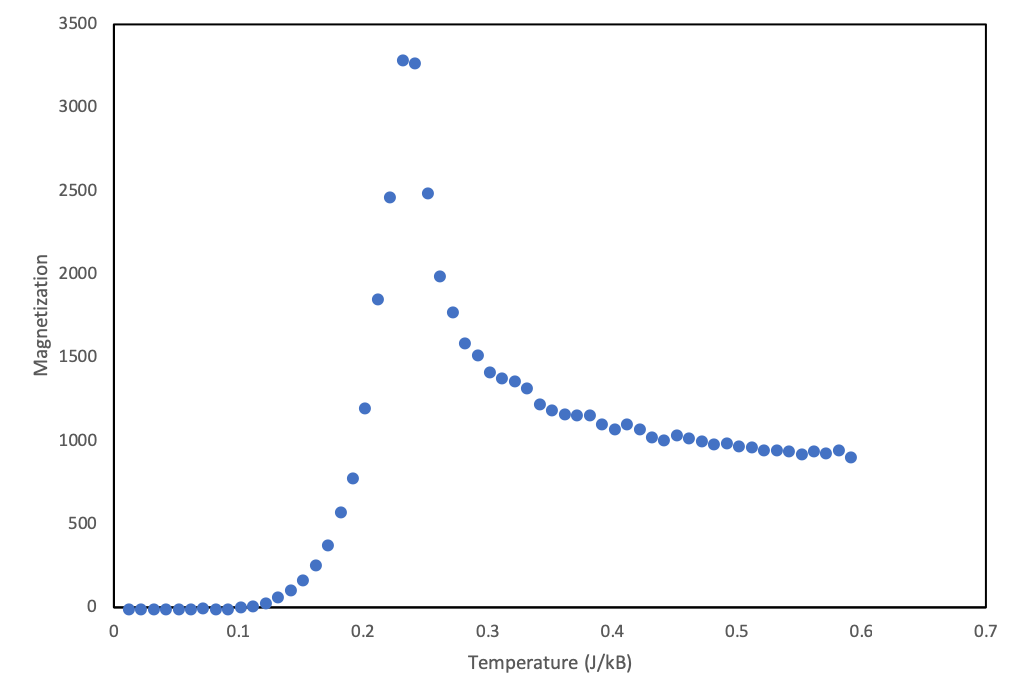
\includegraphics[scale=0.5]{Cv}
				\caption{$C_V$ versus temperature}
		\end{figure}
		




\subsection*{Part b}

	$C_V$ is defined in statisitcal mechanics for the canonical ensamble as \


		\[C_V = (\frac{\partial E}{\partial T})_{N,V}\]

		\[E = -(\frac{\partial \ln Z}{\partial \beta})_{N,V}\]

		\[F = -k_BT \ln Z\]

		\[C_V \propto (\frac{\partial ^2 F}{\partial T^2})_{N,V}\]

	We can look at the graph of $C_V$ to see whether the phase transition is second order. In Figure 14, we can see there is a divergence at around 2.3 $J/k_B$. Which means the ferromagnetic order-disorder transition is classified as a second order transition.


\subsection*{Part c}

	We need to solve for the value of n in the relationship for the Curie Temperature for our value of J. $T_C$ in our case is the point where $C_V$ diverges or the inflection point of the ensamble average magnetization per particle. We can find this graphically from our five independant trials by taking an average. I get $T = 2.3$.

	\[ T_C = \frac{nJ}{k_B}\]

	\[T_C = 2.3 = \frac{nJ}{k_B}\] 

	The Onsager solution is given by 

	\[T_C = \frac{2J}{k \ln (1 + \sqrt{2})}\]

	so $T_C = \frac{2}{k \ln (1 + \sqrt{2})} = 2.269185...$ which is very similar to what was approximated by the simulations $T_C = 2.3$


\subsection*{Part d}
	Above the Curie temperature the magnetization is zero, meaning we have equal number of positive and negative spins in our system. Below the Curie temperature the absolute value of the magnetization per particle is 1 which means that all the spins are alligned in one direction. If the Temperature is above the Curie temperature, the J value is insignificant to determining the order/disorder transition and the temperature dominates (e.g. when calculating alpha, the exponential term dominates the energy difference term). Essentially as temperature increases, the entropy increases and we are more likely to enter disordered states and at long times the system is disordered. 

\newpage

\section*{Problem 3}


\subsection*{Part a}

	The approximate number of timesteps for the system to reach equilibrium is around 500 timesteps ($\Delta T = 0.001$ sampled every 50 timesteps). The plots of kinetic energy, potential energy, and total energy are shown below. See source code for actual implimentation of the MD simulation. The kinetic energy increases sharply, potential energy decreases sharply, but because of the conservation of energy, the total energy remains constant.

	\begin{figure}[H]
				\centering
				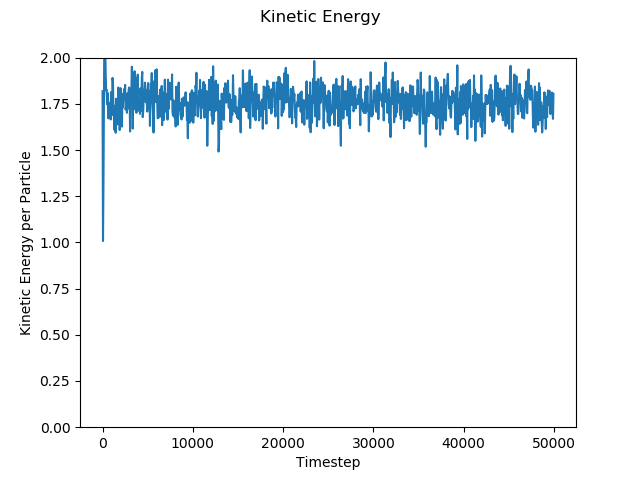
\includegraphics[scale=0.5]{kin_energy}
				\caption{Kinetic energy per particle for 50,000 timesteps and 125 particles}
	\end{figure}

	\begin{figure}[H]
				\centering
				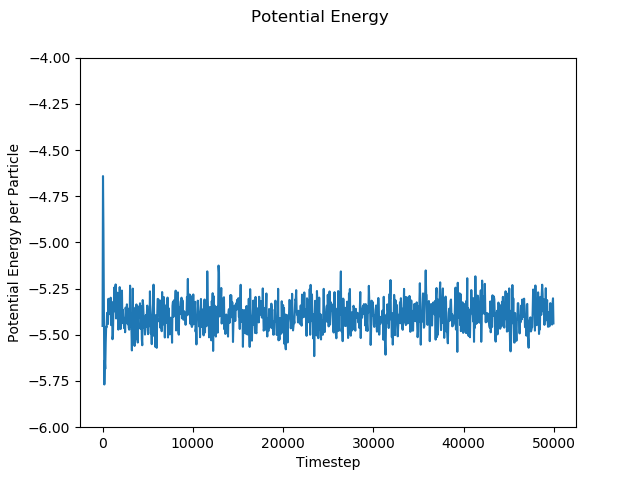
\includegraphics[scale=0.5]{pot_energy}
				\caption{Potential energy per particle for 50,000 timesteps and 125 particles}
	\end{figure}

	\begin{figure}[H]
				\centering
				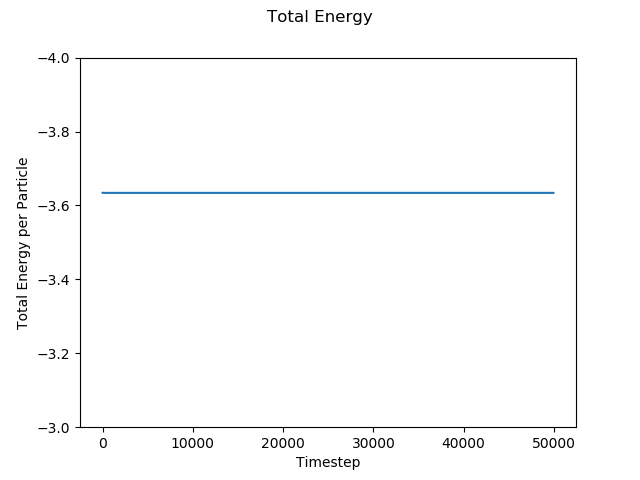
\includegraphics[scale=0.5]{tot_energy}
				\caption{Total energy per particle for 50,000 timesteps and 125 particles}
	\end{figure}
		

\subsection*{Part b}

	Now the total energy will change because we are including the Andersen Thermostat. Plots of the kinetic, potential, and total energy are shown below. The difference compared to part a is that the total energy now has fluctuations because we are using the Andersen Thermostat to hold the temperature constant and energy is being exchanged with the surrounding bath. The exchange of energy is stochastic in nature. The total time to reach thermal equilibrium can be viewed in a temperature per time plot and the time to reach equilibrium was still around 500 timesteps. Compared to part a, the time to reach equilibrium is relativley the same, but the temperature stays constant (besides the fluctuations) when using the Andersen thermostat. Kinetic and Potential energy have the same trend, but total energy now has small fluctuations due to changing individual velocities when they collide with the bath.

 

 	\begin{figure}[H]
				\centering
				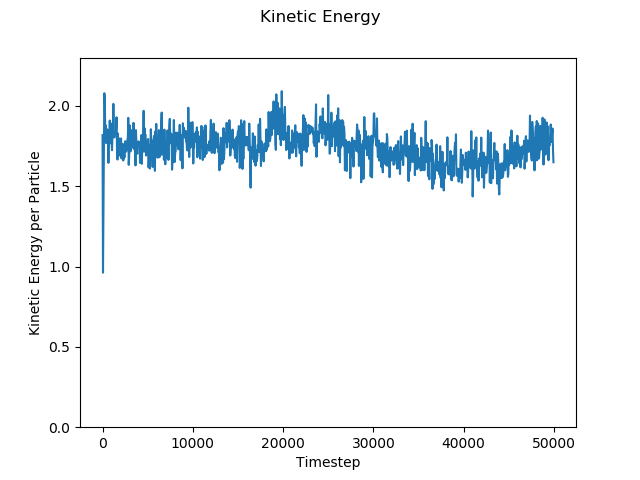
\includegraphics[scale=0.5]{kin_energy_b}
				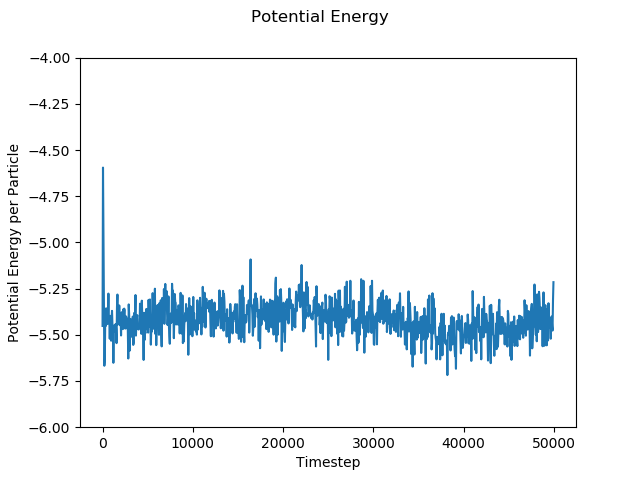
\includegraphics[scale=0.5]{pot_energy_b}
				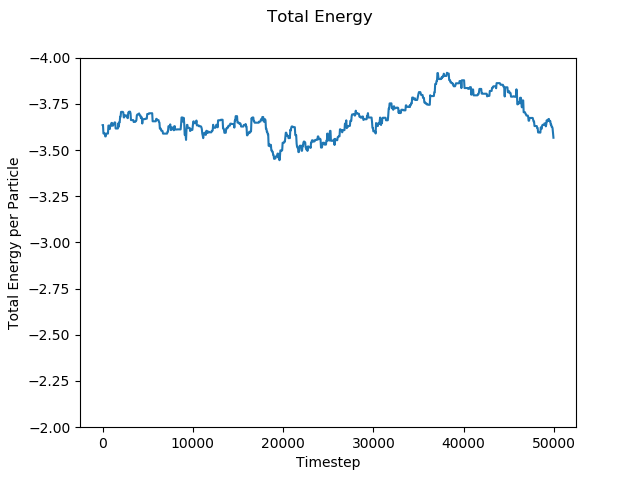
\includegraphics[scale=0.5]{tot_energy_b}
				\caption{Individual plots of energy per particle for 50,000 timesteps and 125 particles}
	\end{figure}

	\begin{figure}[H]
				\centering
				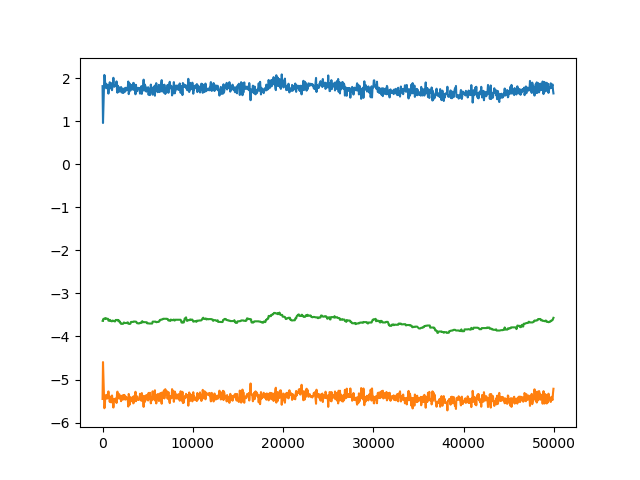
\includegraphics[scale=0.5]{together_b}
				\caption{Combined plot for energy per particle for 50,000 timesteps and 125 particles}
	\end{figure}


\subsection*{Part c}

	Below are histograms for the particle speeds for both the thermostat and non-thermostat cases. I used a time interval of 5,000 timesteps after the system had reached equilibrium, an interval of (30,000 to 35,000). We expect the speed distribution to follow a Maxwell-Boltzman distribution:

	\[\rho (v) = (\frac{m}{2 \pi k_B T})^{3/2} 4 \pi v^2 exp(- \frac{mv^2}{2k_BT})\]

	with mean and variance that we can calculate with the values provided in the problem statement of $k_B = 1$ , $m = 1$, $T = 1.2 \epsilon / k_B$:

	\[\langle v \rangle = \sqrt{\frac{8k_BT}{\pi m}} = 1.748\]

	\[Var(v) = \langle v^2 \rangle - \langle v \rangle ^2 = \frac{k_BT(3 \pi - 8)}{\pi m} = 0.544\]

	\begin{figure}[H]
				\centering
				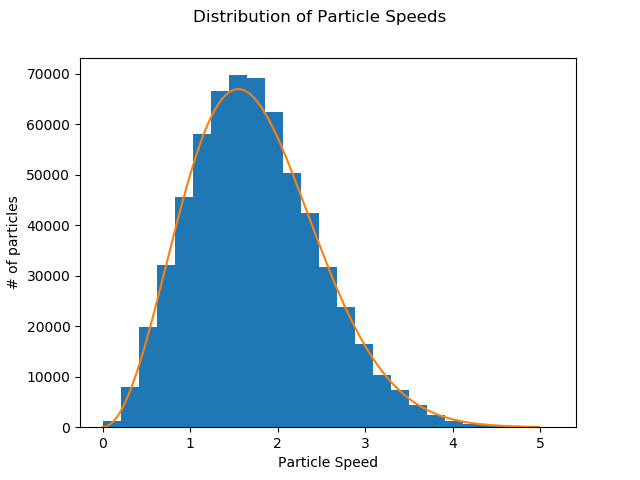
\includegraphics[scale=0.5]{speeds_nothermo}
				\caption{Histogram of the particle speeds with the Maxwell Boltzman distribution overlayed using no thermostat}
	\end{figure}


	The average and variance of the data used to plot the specific histogram above were calculated as $\langle v \rangle = 1.730$ and $Var(v) = 0.523$ with an ensamble average temperature of $1.164 \epsilon / k_B$. I also took an average over three independant trials and got $\langle v \rangle = 1.731$ and $Var(v) = 0.525$ with an ensamble average temperature of $1.162 \epsilon / k_B$


	\begin{figure}[H]
				\centering
				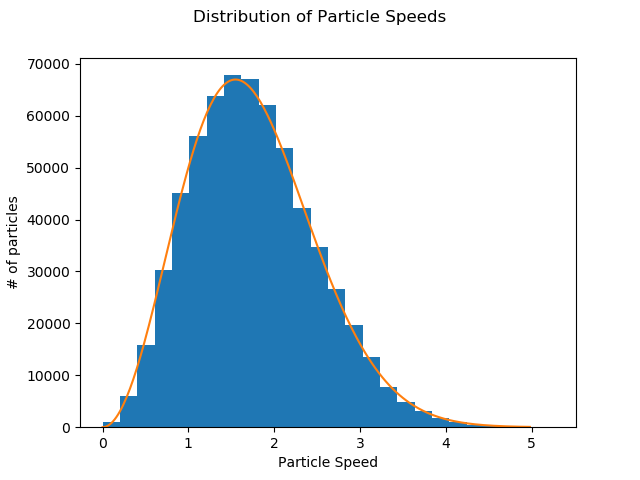
\includegraphics[scale=0.5]{speeds}
				\caption{Histogram of the particle speeds with the Maxwell Boltzman distribution overlayed using the Andersen Thermostat}
	\end{figure}


	The average and variance of the data used to plot the specific histogram above were calculated as $\langle v \rangle = 1.756$ and $Var(v) = 0.530$ with an ensamble average temperature of $1.204 \epsilon / k_B$. I also took an average over three independant trials and got $\langle v \rangle = 1.752$ and $Var(v) = 0.530$ with an ensamble average temperature of $1.201 \epsilon / k_B$  \\

	The results for the cases using the thermostat seem to more closely follow the expected Maxwell Boltzman distribution. This is expected because the Andersen Thermostat keeps the temperature of the system constant and the Maxwell Boltzmann distribution assumes we are in the canonical ensamble (N,V,T). The non-thermostated system however, does not have a constant temperature and over the timesteps sampled the average temperature is not close to the desired temperature and is not constant.

\subsection*{Part d}

	Radial distribution functions were calculated using the algorithm provided in the fluid structure notes and normalized accordingly. below are plots of the radial distribution functions for three different densities. A bin size of 0.02 $\sigma$ was used and the length scale plotted is the maximum distance from particle to particle according to the minimum image convention which is the norm of the box length divided by 2 (corner to center box distance). For a density of 0.85, the radial distribution function is characteristic of a liquid with some exluded volume followed by oscillations showing the solution shells around the reference particle. For a density of 0.10, the radial distribution function is characteristic of a real gas with an excluded volume and one peak that decays smoothly. For a density of 0.01, the system behaves like the density of 0.1 but g(r) decays faster and the peak is narrower. We expect the radial distribution function to level off to 1 in each of these cases, but, since we are only considering one box with the minimum image, g(r) decays to zero. The behavior we are interested in is only the behavior up to the point before the distribution tails off to zero.

		\begin{figure}[H]
				\centering
				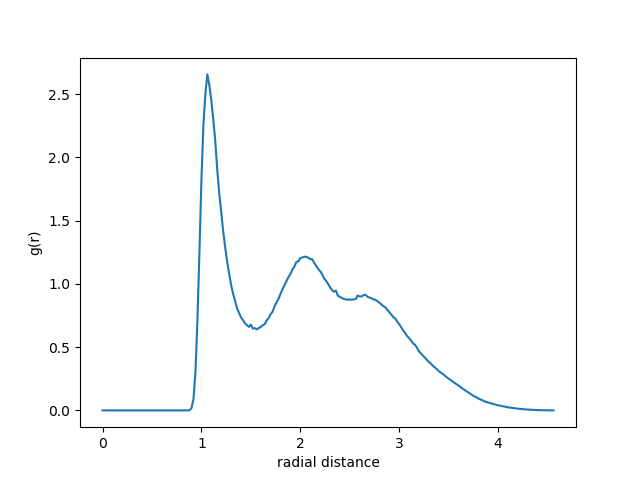
\includegraphics[scale=0.5]{gofr_85}
				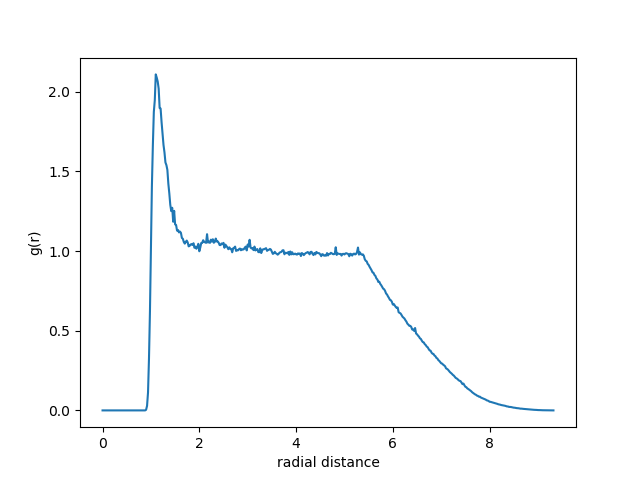
\includegraphics[scale=0.5]{gofr_10}
				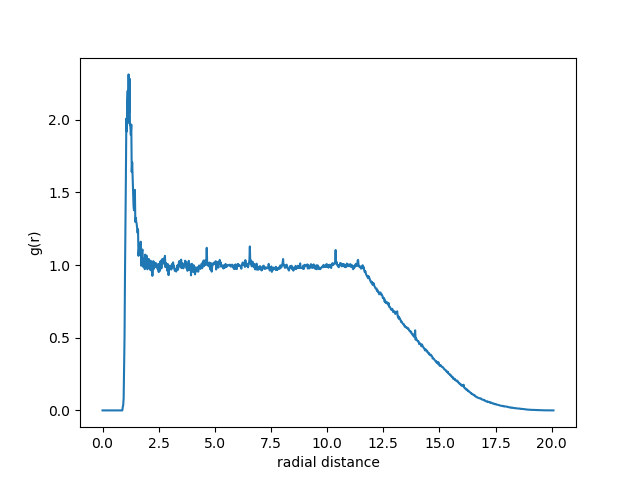
\includegraphics[scale=0.5]{gofr_01}
				\caption{Radial distribution functions for three different densities (from left to right 0.85, 0.1, 0.01)}
		\end{figure}


	BONUS: I wanted to see what the system would look like for a much higher density and see the corresponding radial distribution function for a solid. Shown below is the configuration of particles at equilibrium and the radial distribution function.

		\begin{figure}[H]
				\centering
				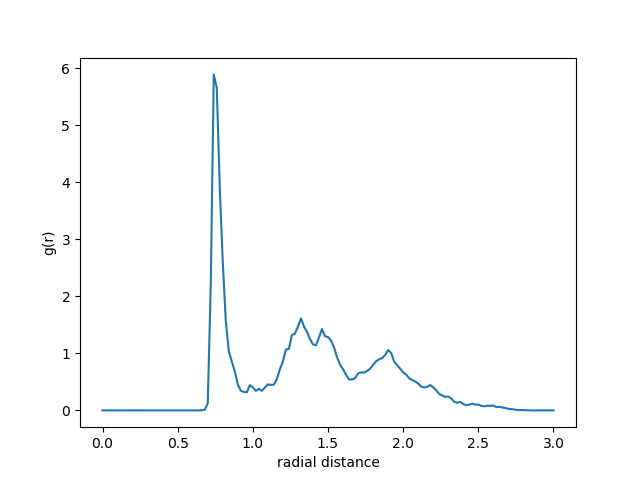
\includegraphics[scale=0.5]{gofr_300}
				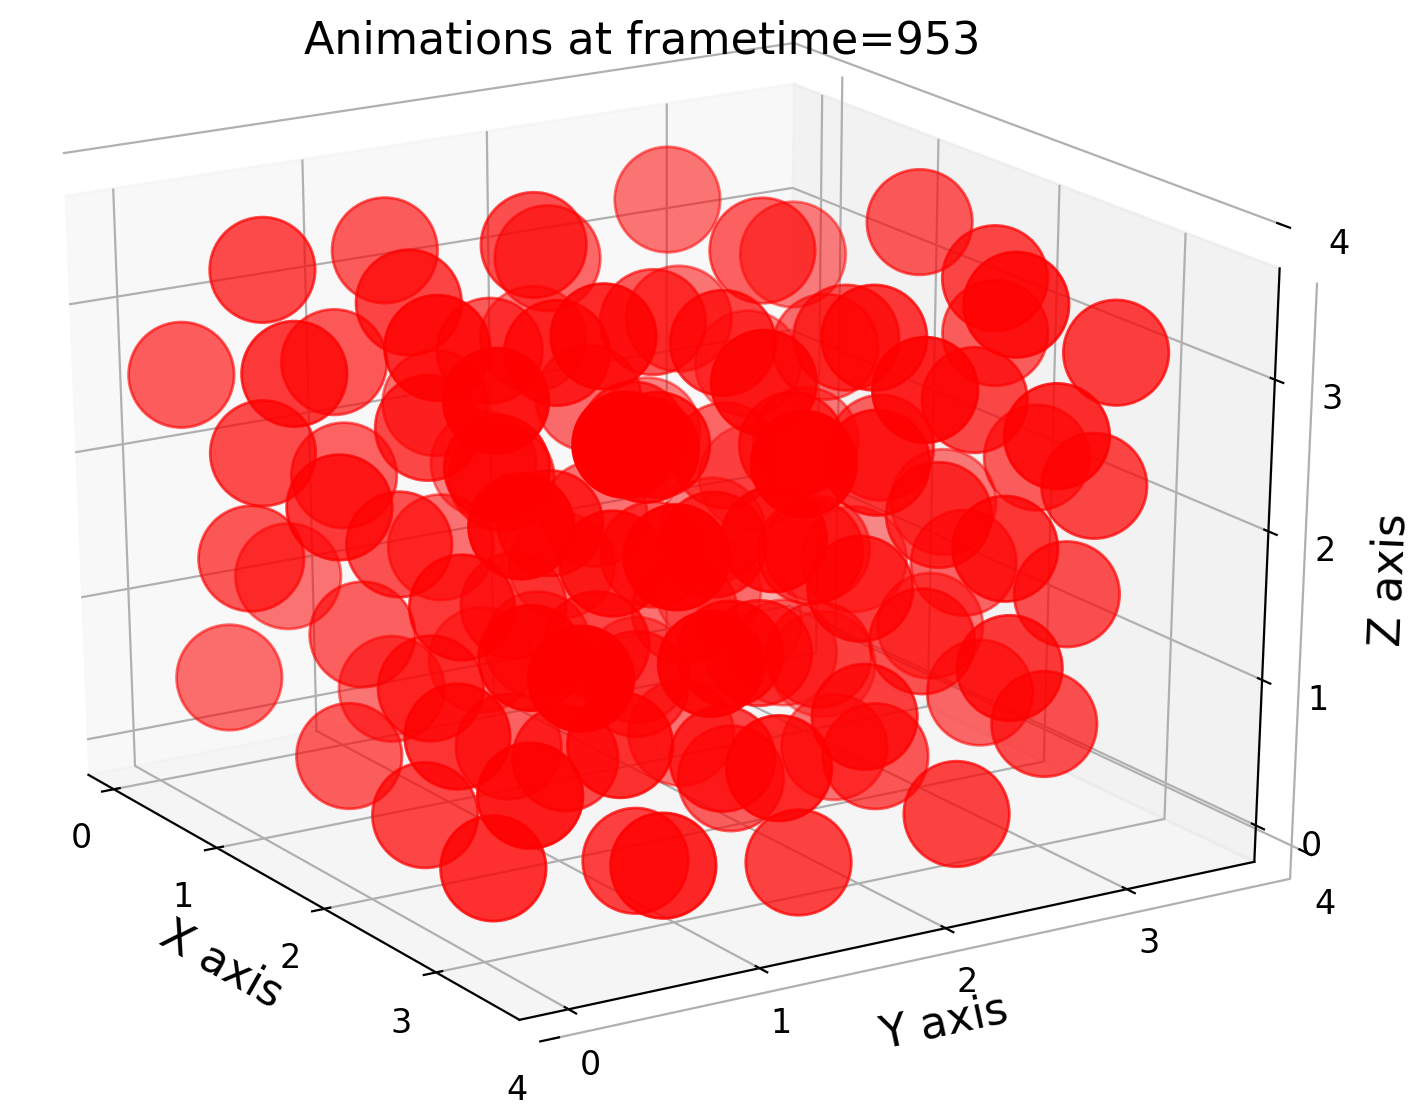
\includegraphics[scale=0.35]{gofr_config}
				\caption{Radial distribution functions for density of 3.0}
		\end{figure}



\subsection*{Part e}
	I initialized the system with particles segregated into two blocks, one of type 1 and one of type 2. I ran the simulation for 100,000 timesteps to ensure I reached equilibrium. Plotted below is the density as a function of z-distance for interaction parameters $\epsilon_22$ equal to 1.0, 3.0, 5.0, 7.0, and 9.0. The blue line corresponds to particles of type 1, and the orange line corresponds to particles of type 2.

		\begin{figure}[H]
				\centering
				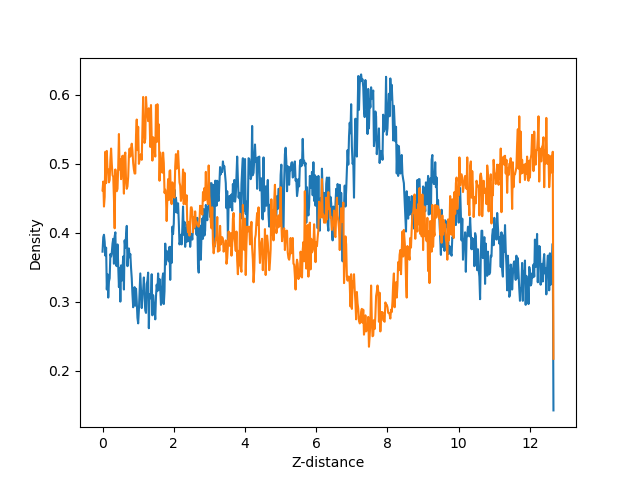
\includegraphics[scale=0.5]{dens_eps1}
				\caption{Density distribution for $\epsilon _{22} = 1$}
		\end{figure}

		The simulation for $\epsilon _{22}=1$ was run for 1,000,000 timesteps to ensure the system mixed. Because both $\epsilon _{11}=1$ and $\epsilon _{22}=1$, the particles are homogeneous and mix completely. The plot of density vs z distance shows a relativley constant density for both types of particles of around 0.42 particles per sigma, which when added, give the bulk density of 0.85 as expected. 

		\begin{figure}[H]
				\centering
				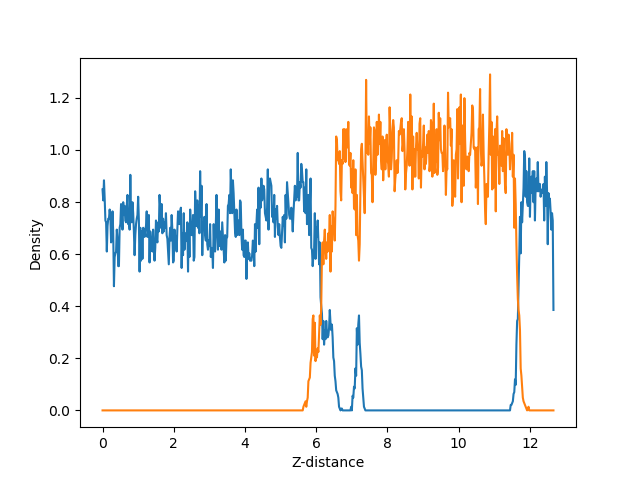
\includegraphics[scale=0.5]{dens_eps3}
				\caption{Radial distribution functions for density of 3.0}
		\end{figure}

		For an  $\epsilon _{22}=3$ the two particles segregate into two phases. There is mixing at the boundaries where you can see the density plots crossing in the plot above. Unlike the cases for $\epsilon _{22}=7$ and $\epsilon _{22}=9$ there is mixing of particle types for long time simulations. The particles do not coordinate into a well defined lattice structure when vizualizing the final configurations. This is essentially two seperate fluid phases with different densities.


		\begin{figure}[H]
				\centering
				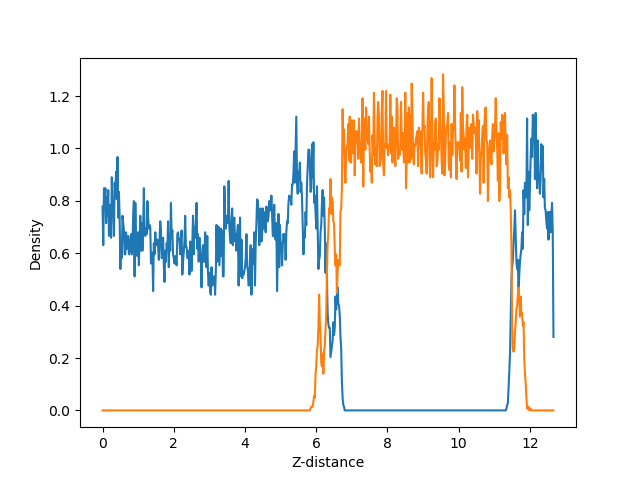
\includegraphics[scale=0.5]{dens_eps5}
				\caption{Radial distribution functions for density of 3.0}
		\end{figure}

		For an  $\epsilon _{22}=5$ the two particles segregate into two phases. There is slight mixing at the boundaries where you can see the density plots crossing in the plot above. Unlike the cases for $\epsilon _{22}=1$ and $\epsilon _{22}=3$ there is less mixing of particle types for long time simulations. The particles do not coordinate into a well defined lattice structure when vizualizing the final configurations


		\begin{figure}[H]
				\centering
				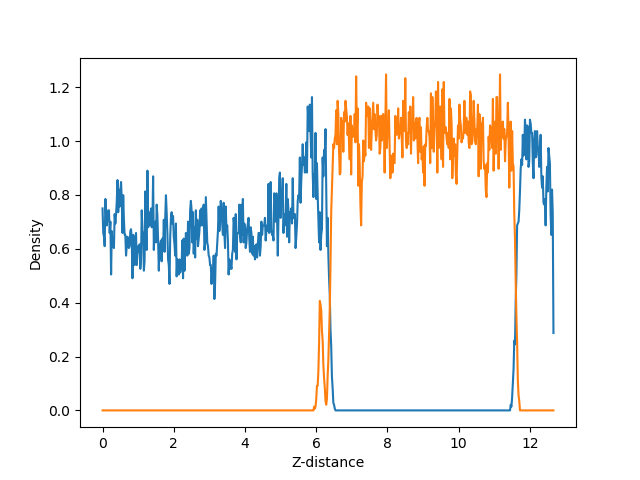
\includegraphics[scale=0.5]{dens_eps7}
				\caption{Density distribution for $\epsilon _{22} = 7$}
		\end{figure}

		For an  $\epsilon _{22}=7$ the two particles segregate into two phases. There are some boundary effects where the density of particles of type one increase because they coordinate to type two particles because of the larger interaction energy. Unlike the cases for $\epsilon _{22}=1$ and $\epsilon _{22}=3$ there is no mixing of particle types at all for long time simulations.


		\begin{figure}[H]
				\centering
				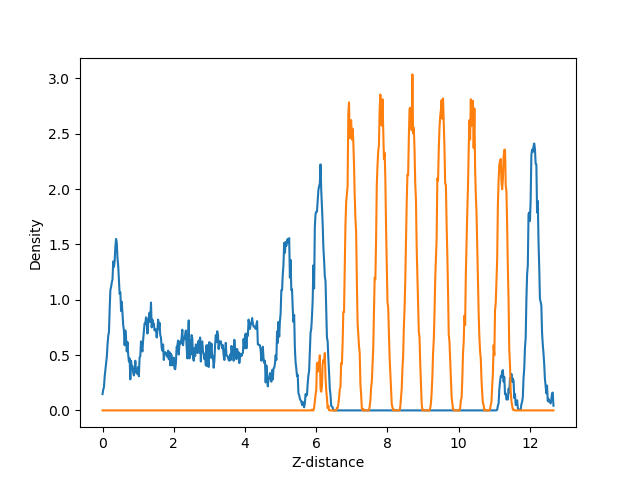
\includegraphics[scale=0.5]{dens_eps9}
				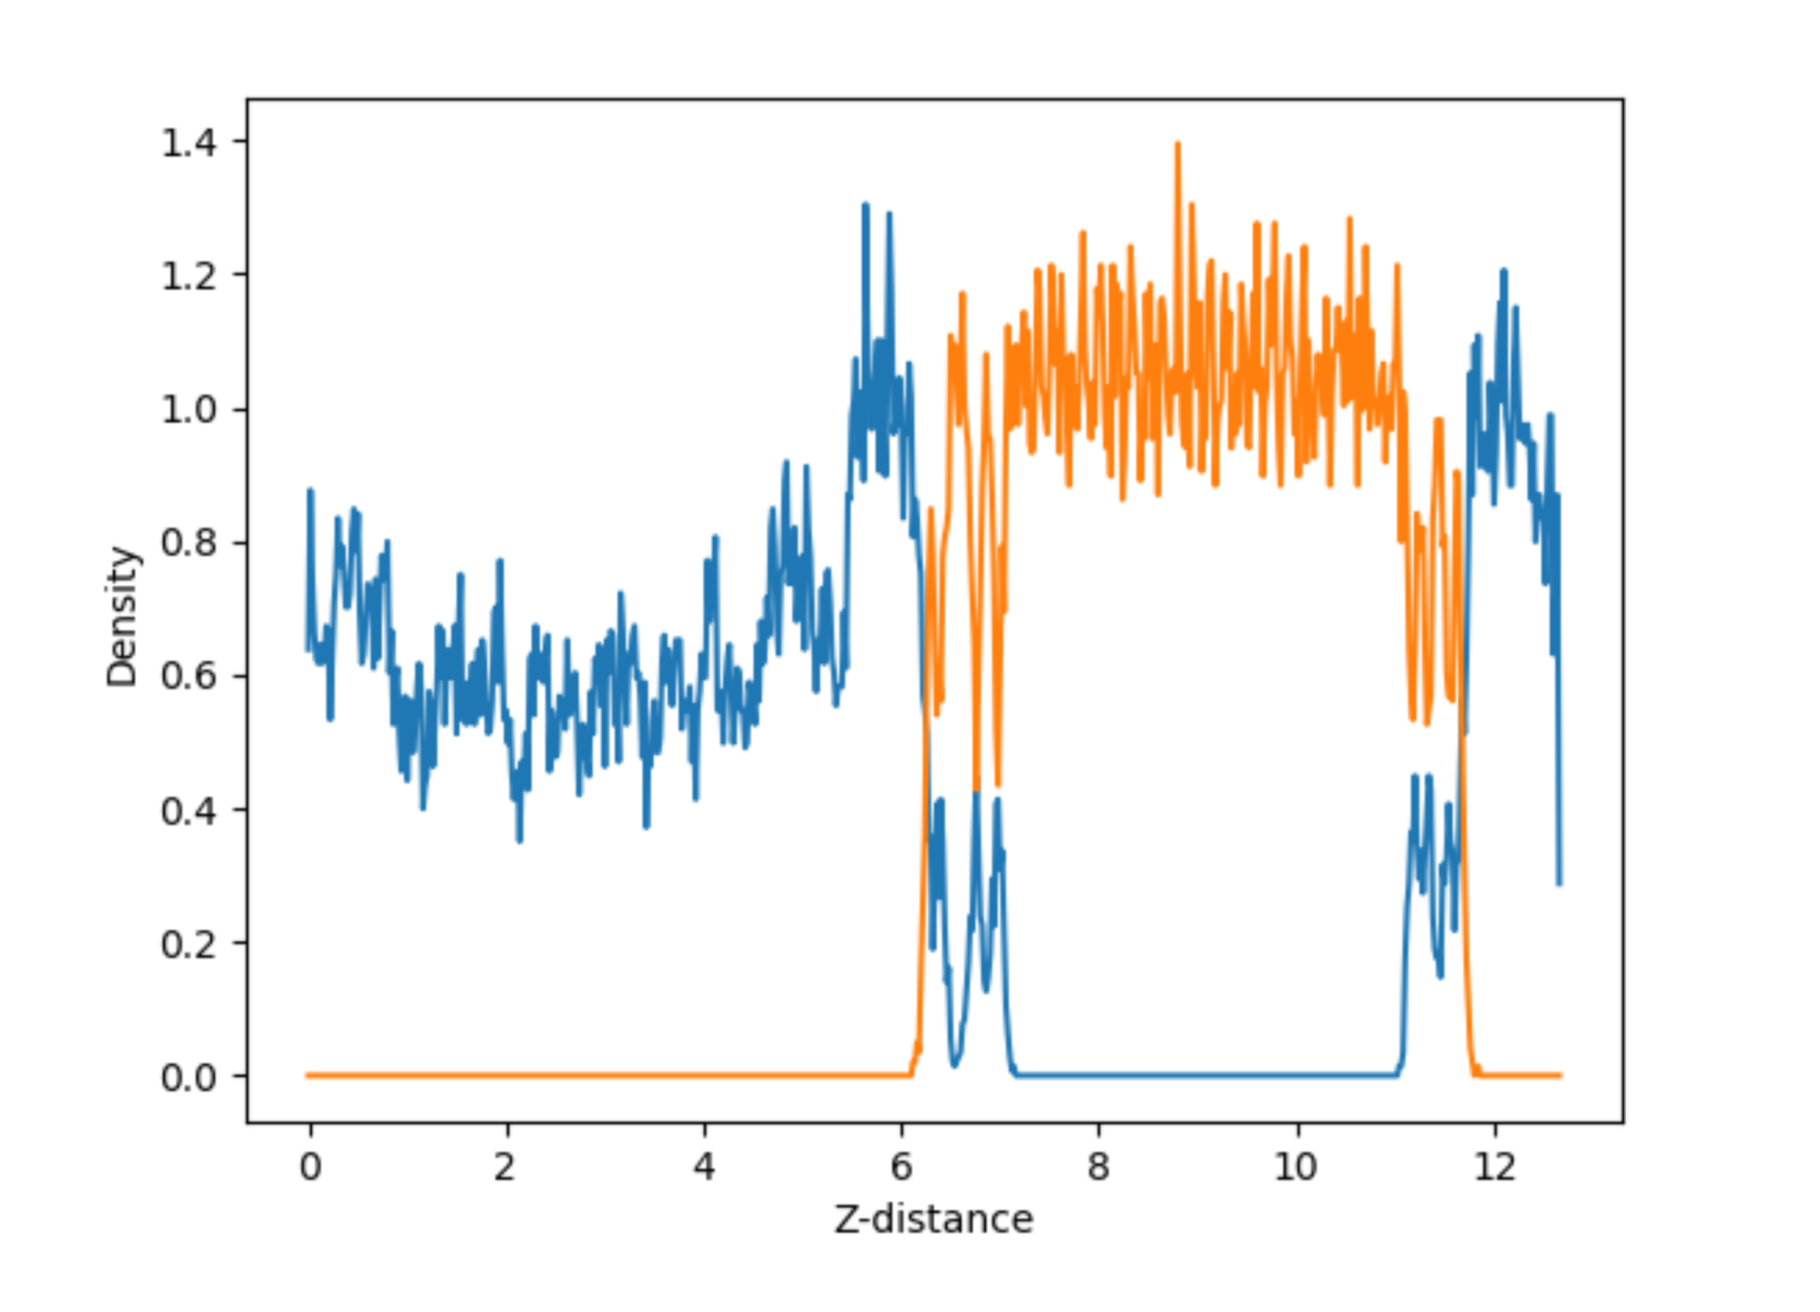
\includegraphics[scale=0.25]{dens_eps9-2}
				\caption{Density distribution for $\epsilon _{22} = 9$}
		\end{figure}

		\begin{figure}[H]
				\centering
				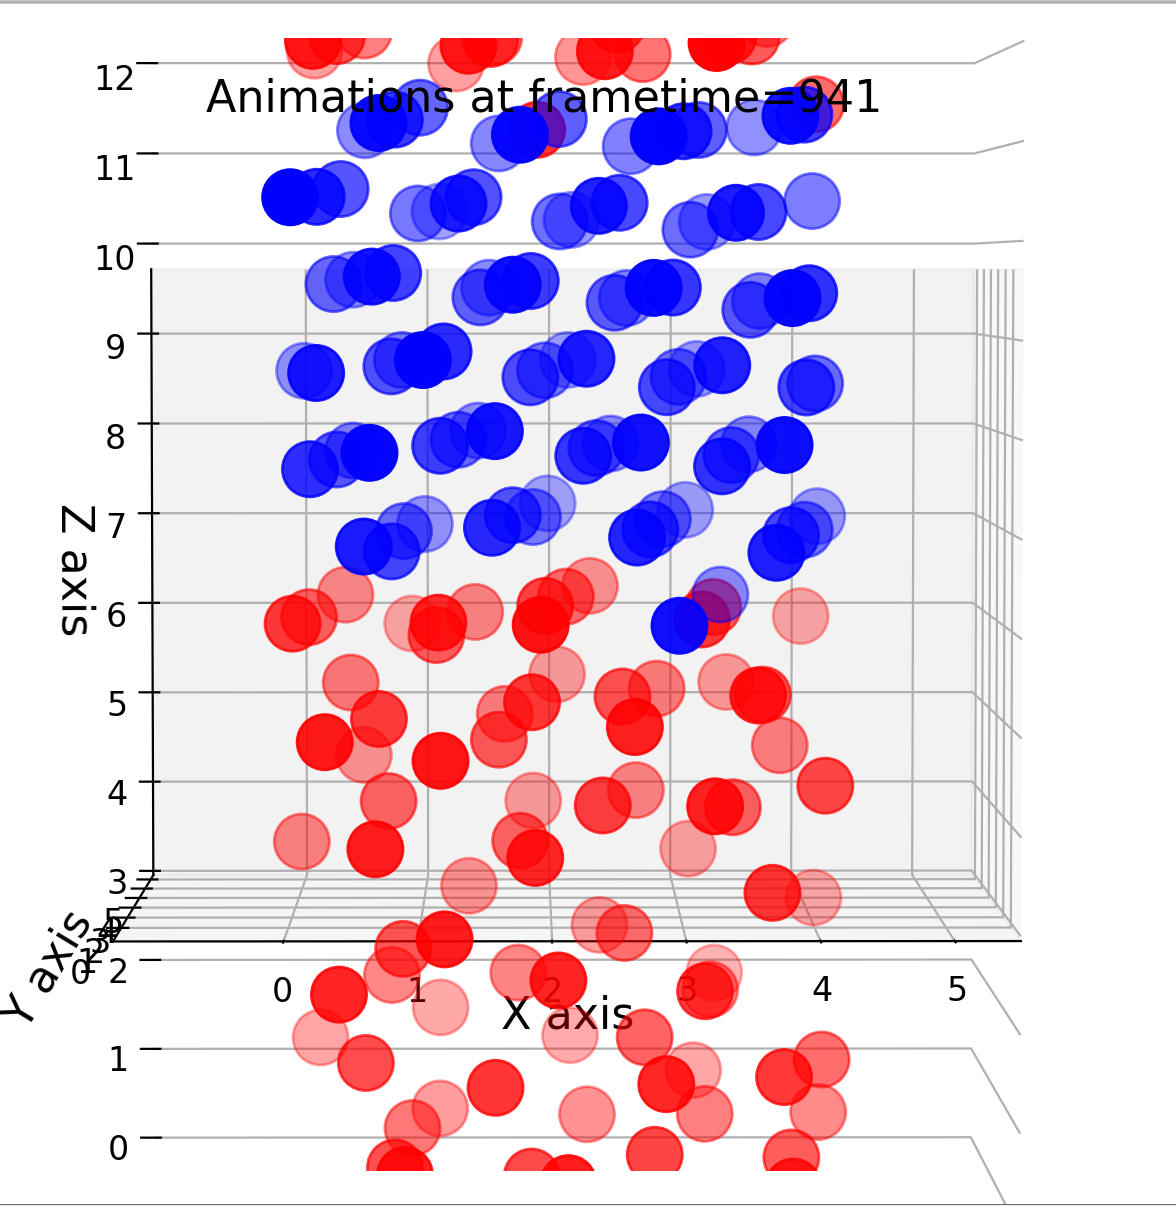
\includegraphics[scale=0.3]{config-9-2}
				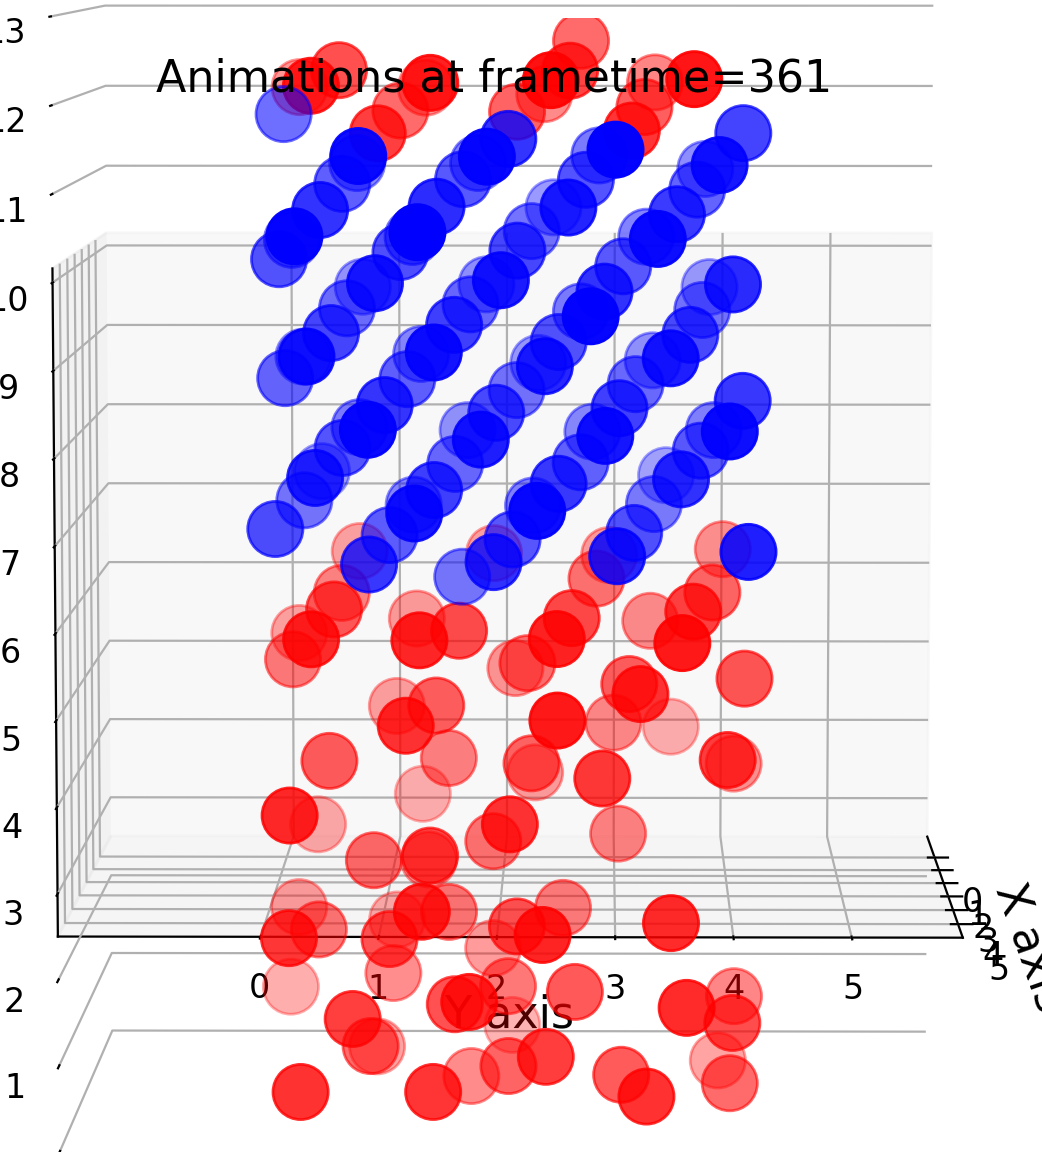
\includegraphics[scale=0.3]{config-9-1}
				\caption{Visualization of converged particle positions both with $\epsilon _{22}=9$}
		\end{figure}


		For an  $\epsilon _{22}=9$ there are multiple steady states that I observed. Shown above are two of the possible states. The particles of type two form a solid phase in a lattice. The orientation of this lattice determines the shape of the density vs. z plot. If the lattice is orthogonal to the z direction you get sharp peaks of density corresponding to the layers of the lattice. If the lattice is non-orthogonal to the z-direction you get a block of constant density of type two with 0 density of type one in the region occupied by particles of type two, and a constant density region of particles of type 1 with 0 density of type two in the region occupied by particles of type 1. At the interface of the two regions we see a spike in density of the liquid phase particles as they are coordinated to the particles with stronger $\epsilon _{12}$ interactions.



\newpage

\section*{Appendix A - Problem 1}

\begin{lstlisting}[language=Python]
# -*- coding: utf-8 -*-
"""
Eric O'Neill 2018 CBE 710 simulation project
"""
#import needed libraries
import Ising_MC_functions as jon
import numpy as np
import random
import matplotlib.pyplot as plt

"""///////////////////////////////FUNCTIONS/////////////////////////////////"""

#this function calculates the total energy of a lattice.
#it assumes there is no external magnetic field H=0.
# E = -sum_i^N mu*H*s_i - (J/2)sum_i^N sum_j^` s_i*s_j
def Calculate_E(tot_num_lattice, pos, neighbors, spins, nearest_neighbors, J):
    #set the energy J, nearest neighbor numbers, and initialize the energy
    energy = 0
    #for each point on the lattice 
    for i in range(tot_num_lattice):
        #iterate over each points nearest neighbors to calculate energies
        for j in range(nearest_neighbors):
            #spin of the current lattice site times the spin of its neighbor
            #for all of the nearest neighbors
            energy += spins[i]*spins[neighbors[i,j]]
    #the final energy is scaled by J and divided by 2 to exclude double counting
    energy = energy * -J/2
    return energy





# this function calculates the change in energy by changing the orientation of 
# one spin
def Delta_E(tot_num_lattice, site_index, neighbors, spins, nearest_neighbors, J):
    #initialize the change in energy due to change in spin
    dE = 0
    #loop over the lattice site's nearest neighbors
    for j in range(nearest_neighbors):
        # for each nearest neighbor, flip the spin s_i and calculate 
        # the energy contribution due to that site and its neighbors
        dE = dE - spins[site_index]*spins[neighbors[site_index,j]]
    # The change in energy due to flipping one spin is dE = Enew - Eold
    # Eold = -Enew in our case so dE = 2*Enew    
    dE = -J * dE * 2
    return dE





# this function calculates the probability of moving to the new state given 
# the old energy and the new energy
def Calculate_alpha(E_old, E_new):
    #Take the min(1,exp(-beta(Enew-Eold)))
    if 1 <= np.exp(-E_new + E_old):
        return 1
    else:
        return np.exp(-E_new + E_old)
"""/////////////////////////////////////////////////////////////////////////"""




"""///////////////////////////////MAIN//////////////////////////////////////"""

#set the values for J and the nearest neighbors
J = 2
nearest_neighbors = 4

# Assume we start in a configuration rm. We choose this config randomly. 
# Call the functions from Ising_MC_functions.py provided on Canvas
pos,neighbors = jon.AssembleSquareLattice(20, 20)
tot_num_lattice,spins = jon.InitializeLattice(20,20)

#Calculate the total energy of the system
energy = Calculate_E(tot_num_lattice, pos, neighbors, spins, nearest_neighbors, J)

#initialize the vector for plotting energy and magnetization
energy_plot_x = [0]
energy_plot_y = [energy/tot_num_lattice]
mag_plot_x = [0]
mag_plot_y = [sum(spins)/tot_num_lattice]

#monte-carlo steps and sampling time
steps = 500000
sample_time = 500

magnetization = 0
energy_avg = 0
energy_squared_avg = 0
count = 0

#iterate over the chosen number of MonteCarlo steps
for i in range(steps):
    #Generate a trial configuration r_n by changing one random spin
    v = random.randint(0, tot_num_lattice-1)
    
    #calculate the change in energy due to flipping one spin
    dE = Delta_E(tot_num_lattice, v, neighbors, spins, nearest_neighbors, J)

    #Calculate how likely we are to accept the new configuration
    alpha = Calculate_alpha(energy, (energy + dE))
    
    #generate a random number to decide if we accept the new config
    u = random.uniform(0, 1)
    
    #accept the new config if u < alpha
    if u < alpha:
        #permanantly change the spin and the total energy
        spins[v] = -spins[v]
        energy = energy + dE
        
        
    #Sample the total energy only certain times
    if (i % sample_time == 0):
        #update the plotting vectors
        energy_plot_x.append(i)
        energy_plot_y.append(energy)
        mag_plot_x.append(i)
        mag_plot_y.append(sum(spins)/tot_num_lattice)
        if i >= 150000:
            energy_avg += energy
            energy_squared_avg += energy*energy
            count = count+1
        
    magnetization = magnetization + sum(spins)
    
    
        
        
        
#plot the results and show the final configurations
   
avg_M = magnetization/steps/tot_num_lattice   

avg_E = energy_avg/count
avg_E2 = energy_squared_avg/count

Cv = (avg_E2 - (avg_E*avg_E))


Cv2 = (np.var(energy_plot_y[301:]))

Cv3 = (np.var(energy_plot_y))

print('average magnetization =' , avg_M)

print('Heat Capacity', Cv)

print('HC CV' , Cv2)
    
print('HC CV' , Cv3)
jon.PlotLatticeConfiguration(pos, spins, 'J=2')   

plt.figure(2)
plt.scatter(energy_plot_x,energy_plot_y) 

plt.figure(3)
plt.scatter(mag_plot_x,mag_plot_y) 

\end{lstlisting}

\newpage

\section*{Appendix B - Problem 2}

\begin{lstlisting}[language=Python]
# -*- coding: utf-8 -*-
"""
Eric O'Neill 2018 CBE 710 simulation project
"""
#import needed libraries
import Ising_MC_functions as jon
import numpy as np
import random
import matplotlib.pyplot as plt

"""///////////////////////////////FUNCTIONS/////////////////////////////////"""

#this function calculates the total energy of a lattice.
#it assumes there is no external magnetic field H=0.
# E = -sum_i^N mu*H*s_i - (J/2)sum_i^N sum_j^` s_i*s_j
def Calculate_E(tot_num_lattice, pos, neighbors, spins, nearest_neighbors, J):
    #set the energy J, nearest neighbor numbers, and initialize the energy
    energy = 0
    #for each point on the lattice 
    for i in range(tot_num_lattice):
        #iterate over each points nearest neighbors to calculate energies
        for j in range(nearest_neighbors):
            #spin of the current lattice site times the spin of its neighbor
            #for all of the nearest neighbors
            energy += spins[i]*spins[neighbors[i,j]]
    #the final energy is scaled by J and divided by 2 to exclude double counting
    energy = energy * -J/2
    return energy





# this function calculates the change in energy by changing the orientation of 
# one spin
def Delta_E(tot_num_lattice, site_index, neighbors, spins, nearest_neighbors, J):
    #initialize the change in energy due to change in spin
    dE = 0
    #loop over the lattice site's nearest neighbors
    for j in range(nearest_neighbors):
        # for each nearest neighbor, flip the spin s_i and calculate 
        # the energy contribution due to that site and its neighbors
        dE = dE - spins[site_index]*spins[neighbors[site_index,j]]
    # The change in energy due to flipping one spin is dE = Enew - Eold
    # Eold = -Enew in our case so dE = 2*Enew    
    dE = -J * dE * 2
    return dE





# this function calculates the probability of moving to the new state given 
# the old energy and the new energy
def Calculate_alpha(E_old, E_new, T):
    #Take the min(1,exp(-beta(Enew-Eold)))
    if 1 <= np.exp((1/T)*(-E_new + E_old)):
        return 1
    else:
        return np.exp((1/T)*(-E_new + E_old))
"""/////////////////////////////////////////////////////////////////////////"""




"""///////////////////////////////MAIN//////////////////////////////////////"""

#initialize plotting vectors
CV_plot_x = np.zeros(60)
CV_plot_y = np.zeros(60)
mag_plot_x = np.zeros(60)
mag_plot_y = np.zeros(60)


 # Assume we start in a configuration rm. We choose this config randomly. 
    # Call the functions from Ising_MC_functions.py provided on Canvas
pos,neighbors = jon.AssembleSquareLattice(20, 20)
tot_num_lattice,spins1 = jon.InitializeLattice(20,20)
l = 0
m = 0

#initial magnetization
sum_spins = sum(spins1)


#iterate over all temperatures
for T in np.arange(0.1,6.0,0.1):
    #set the values for J and the nearest neighbors
    J = 1
    nearest_neighbors = 4
    
    spins = spins1
   
    energy_plot_y = np.zeros(2000)
    
    #Calculate the total energy of the system
    energy = Calculate_E(tot_num_lattice, pos, neighbors, spins, nearest_neighbors, J)
    
    #initialize the vector for plotting energy and magnetization
    
    
    #monte-carlo steps and sampling time
    steps = 1000000
    sample_time = 500
    
    #initialize magnetization and energies
    magnetization = 0
    energy_avg = 0
    energy_squared_avg = 0
    count = 0
    
    k = 0
    
    #iterate over the chosen number of MonteCarlo steps
    for i in range(steps):
        #Generate a trial configuration r_n by changing one random spin
        v = random.randint(0, tot_num_lattice-1)
        
        #calculate the change in energy due to flipping one spin
        dE = Delta_E(tot_num_lattice, v, neighbors, spins, nearest_neighbors, J)
    
        #Calculate how likely we are to accept the new configuration
        alpha = Calculate_alpha(energy, (energy + dE), T)
        
        #generate a random number to decide if we accept the new config
        u = random.uniform(0, 1)
        
        #accept the new config if u < alpha
        if u < alpha:
            #permanantly change the spin and the total energy
            spins[v] = -spins[v]
            sum_spins = sum_spins + 2*(spins[v])
            energy = energy + dE
            
            
            
             #Sample the total energy only certain times
        if (i % sample_time == 0):
            #update the plotting vectors
            energy_plot_y[k] = energy
            k += 1
    
                
            
        #update the magnetization
        magnetization = magnetization + sum_spins
        
            
            
            
    #plot the results and show the final configurations
       
    
    #jon.PlotLatticeConfiguration(pos, spins, 'J=2')  
    avg_M = np.abs(magnetization/steps/tot_num_lattice)
    mag_plot_x[m] = T
    mag_plot_y[m] = avg_M
    
    Cv = (np.var(energy_plot_y[301:]))

    CV_plot_x[m] = T
    CV_plot_y[m] = Cv

    m += 1

    
#jon.PlotLatticeConfiguration(pos, spins, 'J=2')   

plt.figure(2)
plt.plot(mag_plot_x,mag_plot_y) 

plt.figure(3)
plt.plot(CV_plot_x,CV_plot_y) 



\end{lstlisting}

\newpage

\section*{Appendix C - Problem 3}

\begin{lstlisting}
#!/usr/bin/env python3
# -*- coding: utf-8 -*-
"""
Created on Mon Oct 22 13:54:47 2018

@author: oneill
"""
import MD_functions as MD
import numpy as np
import matplotlib.pyplot as plt
import time
import random



#this function calculates the forces between all particles and returns an 
#nxnx3 array of the forces and the potential energy of the system. find the force
#experienced by particle i by summing the ith row of the array
def CalculateForces2(pos, epsilon, sigma, num_particles, L):
    
    #initialize force vector, potential energy, vector of x,y,z distances
    #and the actual distance
    forces = np.zeros([num_particles, num_particles, 3])
    pot_energy = 0
    delxyz = np.zeros([num_particles,num_particles, 3])
    rij = np.zeros([num_particles,num_particles])
            
    
    #use broadcasting arrays to make an nxnx3 array containing the x-x, y-y, z-z distances
    #for all pairs of particles, this also implements the minimum image convention
    #to calculate the x,y,z distance w.r.t the periodic boundary conditions
    delxyz = (pos[np.newaxis,:,:] - pos[:,np.newaxis,:]) - np.rint((pos[np.newaxis,:,:] - 
    pos[:,np.newaxis,:])/L)*L
    
    #use broadcasting arrays to make an nxn array containing the distances btwn all particles
    rij = np.linalg.norm(delxyz, axis=2)
    
    #square the distances for use in force eqns below
    rij = rij**2
    
    #turn 0s to 1 because dividing by 0 causes trouble... 
    rij[rij == 0] = 1
    
    #calculate the forces in the three directions
    forces[:,:,0] = -(48*epsilon/rij)*((sigma**12)/(rij**6)  -  
    (0.5)*((sigma**6)/(rij**3)))*delxyz[:,:,0]

    forces[:,:,1] = -(48*epsilon/rij)*((sigma**12)/(rij**6)  -  
    (0.5)*((sigma**6)/(rij**3)))*delxyz[:,:,1]

    forces[:,:,2] = -(48*epsilon/rij)*((sigma**12)/(rij**6)  -  
    (0.5)*((sigma**6)/(rij**3)))*delxyz[:,:,2]
    
    #calculate the potential energy and divide by 2 to avoid overcounting
    pot_energy = 0.5*np.sum(4*epsilon*((sigma**12)/(rij**6)  -  ((sigma**6)/(rij**3))))
    
    
    return forces, pot_energy

#this function calculates the new positions of particles and returns an nx3 array of 
#particle positions. 
def NewPositions(pos, vels, forces, timestep, mass, num_particles, L):
    
    #uses the equation from notes to calculate new positions.
    #sum along first axis of force array to get forces.
    pos = pos + vels*timestep + 0.5*mass*np.sum(forces, axis=1)*timestep*timestep
   
    #implement the periodic boundary conditions for all three directions
    pos[:,0] = pos[:,0] - np.floor(pos[:,0]/L[0])*L[0]
    pos[:,1] = pos[:,1] - np.floor(pos[:,1]/L[1])*L[1]
    pos[:,2] = pos[:,2] - np.floor(pos[:,2]/L[2])*L[2]
    
    return pos

#This function computes the half velocity step. returns an nx3 array of particle
#half velocities
def HalfVelocity(vels, mass, timestep, forces, num_particles):
    
    #initialize half velocity vector
    halfvels = np.zeros([num_particles, 3])
    #use half step velocity formula
    halfvels = vels + 0.5*mass*np.sum(forces, axis=1)*timestep
    
    return halfvels


#This function computes the velocities of all particles. returns an nx3 array of 
#particle velocities
def UpdateVels(vels, halfvels, mass, timestep, forces, num_particles):
    
    #use velocity formula from notes
    vels = halfvels + 0.5*mass*np.sum(forces, axis=1)*timestep
    
    return vels
    
#this function calculates the Kinetic energy of the system by summing the 
#kinetic energy of each particle. returns a scalar
def KineticEnergy(vels, mass):
    #initialize kinetic energy
    k = 0
    #loop over all velocities and calculate the kinetic energy
    for i in range(len(vels)):
        k += 0.5*mass*(vels[i,0]**2 + vels[i,1]**2 + vels[i,2]**2)
    
    return k


def RadialDist(pos, bins, L, dr, num_particles):
    
    #initialize distance arrays
    delxyz = np.zeros([num_particles,num_particles, 3])
    rij = np.zeros([num_particles,num_particles])
            
    
    #use broadcasting arrays to make an nxnx3 array containing the x-x, y-y, z-z distances
    #for all pairs of particles, this also implements the minimum image convention
    #to calculate the x,y,z distance w.r.t the periodic boundary conditions
    delxyz = (pos[np.newaxis,:,:] - pos[:,np.newaxis,:]) - np.rint((pos[np.newaxis,:,:] -
     pos[:,np.newaxis,:])/L[0])*L[0]
    
    #use broadcasting arrays to make an nxn array containing the distances btwn all particles
    rij = np.linalg.norm(delxyz, axis=2)
    
    #Change to integers so it works as indicies
    rij = np.rint(rij/dr)
    rij = rij.astype(int)
    
    #update histograms
    for i in range(num_particles):
        j = i+1
        while j < num_particles:
            bins[rij[i,j]] += 1
            j+=1
    
    return bins

#this function finds the number of particles in each bin for the current 
#simulation step
def DensityCalc(pos, dens_bins1, dens_bins2, L, dz, num_particles):
        
    for i in range(num_particles):
        #Do it for the two different particle types
        if i < num_particles/2:
            dens_bins1[np.floor(pos[i,2]/dz).astype(int)] += 1
        else:
            dens_bins2[np.floor(pos[i,2]/dz).astype(int)] += 1

    
    return dens_bins1, dens_bins2




"""///////////////////////////////MAIN//////////////////////////////////////"""

#Checking the efficiency of the simulation
start1 = time.time()

#THERMOSTAT
andersen_themostat = 1
collision_frequency = 0.1

#2-particle system
two_particles = 1
epsilon11 = 1.0
epsilon22 = 3.0
epsilon12 = (epsilon11*epsilon22)**(0.5)

#initialize variables#
pos = []
mass = 1
simulation_steps = 80000
#how often to sample system
vid_sample_frames = 50
#how long the plot vectors should be
frames = simulation_steps/vid_sample_frames
timestep = .001
num_particles = 192

#define epsilon for a one or two particle system
if two_particles == 1:
    
    epsilon = np.zeros([num_particles,num_particles])
    for i in range(num_particles):
        for j in range(num_particles):
            if j < num_particles/2 and i < num_particles/2:
                epsilon[i,j] = epsilon11
                
            elif j >= num_particles/2 and i < num_particles/2:
                epsilon[i,j] = epsilon12
                
            elif j < num_particles/2 and i >= num_particles/2:
                epsilon[i,j] = epsilon12
                
            elif j >= num_particles/2 and i >= num_particles/2:
                epsilon[i,j] = epsilon22

else:
    epsilon = 1




kB = 1
density = 0.85
#lattice diamater
sigma = (1/((density)**(1/3)))
#sigma in force eqn
force_sigma = 1
Temp = 1.2*(epsilon11/kB)
pot_energy = 0

#initialize the lattice of particle positions
pos, box_size = MD.AssembleCubeLattice(sigma, density, 4,4,12)

#move the particles off the boundary to start
pos[:,0] = pos[:,0] + 0.001
pos[:,1] = pos[:,1] + 0.001
pos[:,2] = pos[:,2] + 0.001

#initialize the particle velocities
vels = MD.AssignInitialVelocities(Temp,kB, mass, num_particles)

#calculate the initial forces on the particles
forces, pot_energy = CalculateForces2(pos, epsilon, force_sigma, num_particles, box_size)

#initialize animation array
video = np.zeros([int(frames) + 1, num_particles,3])
frame_index = 0


# initialize plotting Variables
KE_plot = np.zeros(int(frames) + 1)
PE_plot = np.zeros(int(frames) + 1)
Total_energy_plot = np.zeros(int(frames) + 1)
time_plot = np.zeros(int(frames) + 1)
Temp_plot = np.zeros(int(frames) + 1)

speed_range_min = 30000
speed_range_max = 35000
speed_index = 0
Speed_plot = np.zeros((speed_range_max - speed_range_min)*num_particles)


#Radial distribution stuff
dr = 0.02
maxdist = (((box_size[0])/2)**2 + ((box_size[1])/2)**2 + ((box_size[2])/2)**2)**(0.5)
bins = np.zeros(int(np.ceil(maxdist/dr) ))

#density z direction stuff
dz = 0.02
dens_bins1 = np.zeros(np.ceil(box_size[2]/dz).astype(int))
dens_bins2 = np.zeros(np.ceil(box_size[2]/dz).astype(int))

#load initial energies and positions into plotting arrays
video[frame_index,:,:] = pos
KE_plot[frame_index] = KineticEnergy(vels, mass)
PE_plot[frame_index] = pot_energy
Total_energy_plot[frame_index] = KE_plot[frame_index] + PE_plot[frame_index]
frame_index += 1


times_vels = 0


#MAIN LOOP

for i in range(0, simulation_steps):
    #calculate the new positions from initial velocities and forces
    pos = NewPositions(pos,vels,forces,timestep,mass,num_particles, box_size)
    
    #calculate the half velocity update
    halfvels = HalfVelocity(vels, mass, timestep, forces, num_particles)
    
    #generate the new forces and calculate the potential energy    
    forces, pot_energy = CalculateForces2(pos, epsilon, force_sigma, num_particles, box_size)

    #finish the velocity update
    vels = UpdateVels(vels, halfvels, mass, timestep, forces, num_particles)
    
    
    #implements the Andersen Thermostat if boolean is true
    if(andersen_themostat == 1):
        for j in range(num_particles):
            v = random.uniform(0, 1)
            if v < collision_frequency*timestep:
                times_vels += 1
                #re-set velocities based on the boltzman distribution with
                #mean = 0 and stdev = sqrt(kT/m)
                vels[j,:] = np.random.randn(3)*(kB*Temp*(1/mass))**(1/2)
                
                
                #remove center of mass velocity from each particle
                com_vel = np.zeros([1, 3])
                for l in range(num_particles):
                    com_vel = com_vel + vels[l, :]
                com_vel = com_vel / num_particles
                for l in range(num_particles):
                    vels[l,:] = vels[l, :] - com_vel
                
                #scale to correct temp
                cur_temp = 0.66 * KineticEnergy(vels,mass) / num_particles
                scale_factor = np.sqrt(Temp /cur_temp) 
                # multiply velocities by scale factor to get new correct temp
                vels = vels*scale_factor
                
    #Calculates and stores the speeds for a converged simulation
    if i > speed_range_min and i < speed_range_max:
        for m in range(len(vels)):
            Speed_plot[speed_index] = np.linalg.norm(vels[m,:])
            speed_index += 1
    
    #sample every x timesteps
    if(i % vid_sample_frames == 0):
        #update plotting arrays
        video[frame_index,:,:] = pos
        KE_plot[frame_index] = KineticEnergy(vels, mass)
        PE_plot[frame_index] = pot_energy
        Temp_plot[frame_index] = 0.66 * KE_plot[frame_index] / num_particles
        Total_energy_plot[frame_index] = KE_plot[frame_index] + PE_plot[frame_index]
        time_plot[frame_index] = i
        frame_index += 1
        
        #density z direction calculations
        if two_particles ==1 and i >= 60000:
            dens_bins1, dens_bins2 = DensityCalc(pos,dens_bins1,dens_bins2,box_size,dz,
            num_particles)
        
        #Radial distribution functions
        #bins = RadialDist(pos,bins,box_size,dr,num_particles)
        
        
#finish timing the simulation
end1 = time.time() 

"""
#Radial distribution normalization
index_set = np.arange(0,len(bins),1)
radial_plotx = np.arange(0,maxdist,0.02)
bins = bins/(simulation_steps/vid_sample_frames) 
bins = bins/num_particles
bins = bins/(4*np.pi/3 * dr**3 * ((index_set + 1)**3 - index_set**3) )
bins = 2*bins/density
  """  
#calculate energy per particle
KE_plot = KE_plot/num_particles
PE_plot = PE_plot/num_particles
Total_energy_plot = Total_energy_plot/num_particles


""" PLOTTING SECTION """

"""
#plot individual graphs
plt.figure(1)
plt.plot(time_plot, KE_plot)
plt.ylabel('Kinetic Energy per Particle')
plt.xlabel('Timestep')
plt.suptitle('Kinetic Energy')
plt.ylim(0,2.3)
plt.show()

plt.figure(2)
plt.plot(time_plot, PE_plot)
plt.ylabel('Potential Energy per Particle')
plt.xlabel('Timestep')
plt.suptitle('Potential Energy')
plt.ylim(-6,-4)
plt.show()

plt.figure(3)
plt.plot(time_plot, Total_energy_plot)
plt.ylabel('Total Energy per Particle')
plt.xlabel('Timestep')
plt.suptitle('Total Energy')
plt.ylim(-2,-4)
plt.show()
"""
#Plot all on one figure
plt.figure(4)
plt.plot(time_plot, KE_plot)
plt.plot(time_plot, PE_plot)
plt.plot(time_plot, Total_energy_plot)
plt.legend('Kinetic Energy' 'Potential Energy' 'Total Energy')



#SPeed Histogram
num_bins = int(np.floor((np.max(Speed_plot) - np.min(Speed_plot))/0.2))
plt.figure(6)
def f(t):
    return (mass/(2*np.pi*kB*Temp))**(3/2) * 4 * np.pi * t**2 * 
    np.exp(-(mass*t**2)/(2*kB*Temp) )


plt.hist(Speed_plot, num_bins)
t = np.arange(0.0,5.0, 0.02)
nnn = f(t)*125000
plt.plot(t,nnn)
print(np.average(Speed_plot))
print(np.var(Speed_plot))
plt.ylabel('# of particles')
plt.xlabel('Particle Speed')
plt.suptitle('Distribution of Particle Speeds')
plt.show()


#plt.figure(7)
#plt.plot(time_plot,Temp_plot)
#plt.show()

#plt.figure(8)
#plt.plot(radial_plotx,bins)
#plt.ylabel('g(r)')
#plt.xlabel('radial distance')
#plt.title('Radial distribution function for density = %' %density)
#plt.show

if two_particles == 1:
    #normalize by the number of samples and the volume of each bin
    dens_bins1 = dens_bins1/((simulation_steps-60000)/vid_sample_frames)
    dens_bins2 = dens_bins2/((simulation_steps-60000)/vid_sample_frames)
    dens_bins1 = dens_bins1/(dz*box_size[0]*box_size[1])
    dens_bins2 = dens_bins2/(dz*box_size[0]*box_size[1])

    #create plotting vector
    z_plotting = np.arange(0,box_size[2],dz)
    plt.figure(9)
    plt.plot(z_plotting, dens_bins1)
    plt.plot(z_plotting,dens_bins2)
    plt.ylabel('Density')
    plt.xlabel('Z-distance')
    plt.show()


avg_T = np.sum(Temp_plot)/len(Temp_plot)

identity = np.ones(num_particles)
for i in range(num_particles):
    if i < num_particles/2:
        identity[i] = 1
    else:
        identity[i] = 0
        
identity.astype(int)

print(avg_T)
print(end1-start1)



\end{lstlisting}





\end{document}